% coding:utf-8

%----------------------------------------
%FOSADSVB, a LaTeX-Code for a summary of digital signal processing
%Copyright (C) 2015, Mario Felder & Michi Fallegger

%This program is free software; you can redistribute it and/or
%modify it under the terms of the GNU General Public License
%as published by the Free Software Foundation; either version 2
%of the License, or (at your option) any later version.

%This program is distributed in the hope that it will be useful,
%but WITHOUT ANY WARRANTY; without even the implied warranty of
%MERCHANTABILITY or FITNESS FOR A PARTICULAR PURPOSE.  See the
%GNU General Public License for more details.
%----------------------------------------

\chapter{Adaptive Filter}
\section{Linear Predictive Coding}
Sprachsignal mit Ordnung $P$ (all-pole filter):
\[ H(z) = \frac{g}{1-\sum_{k=1}^{P}a_kz^{-k}} \]
LPC-10e Algrithmus:
\begin{itemize}
	\item 8000 Samples/s
	\item 180 Samples/Segment
	\item $P=10$
	\item 54 bits pro Segment für Encoding
	\item Bitrate von 2400 bit/s
\end{itemize}
Entscheidet für jedes Segment, ob es voiced oder unvoiced ist. Konsonanten zählen
als unvoiced, da das Signal einem Rauschen gleicht. Vokale erzeugen eine 
periodische Schwingung mit $T_0$.\\
\\
Differenzengleichung
\[ s[n] = \sum_{k=1}^{P}a_ks[n-1] + g \cdot v[n] \]
\begin{minipage}{.5\textwidth}
\begin{center}
	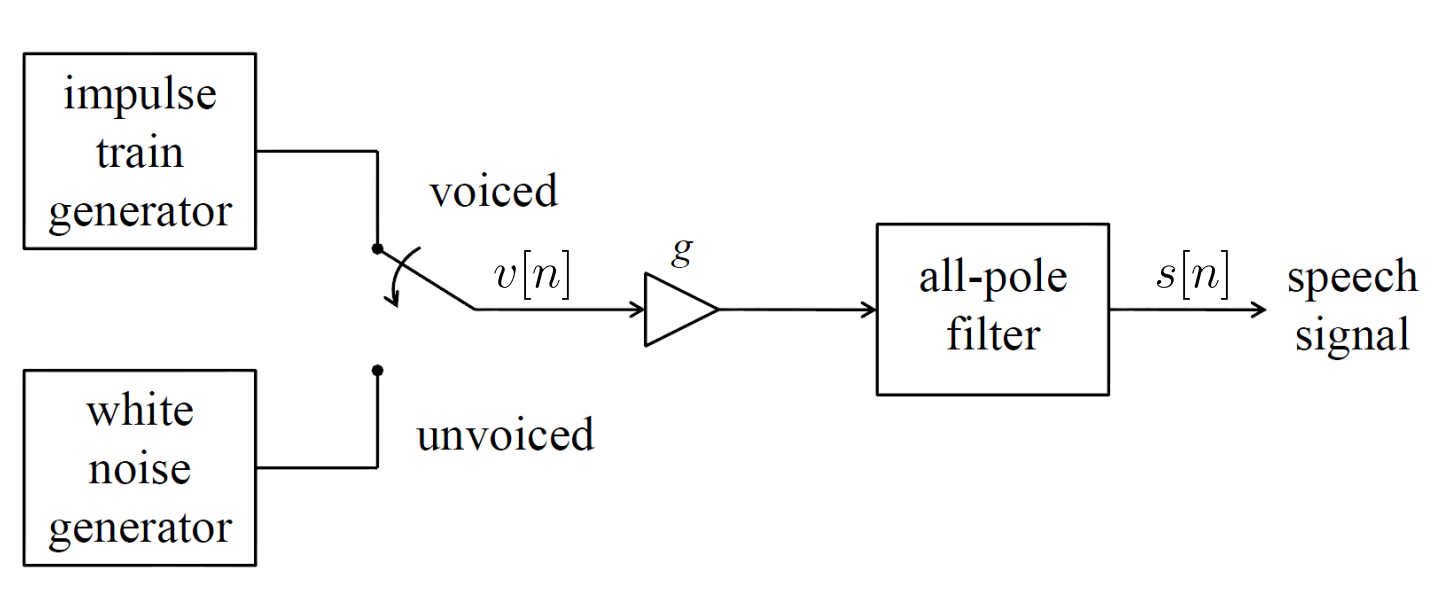
\includegraphics[width=\textwidth]{./images/speech_signal}
\end{center}
\end{minipage}
\begin{minipage}{.5\textwidth}
\begin{center}
	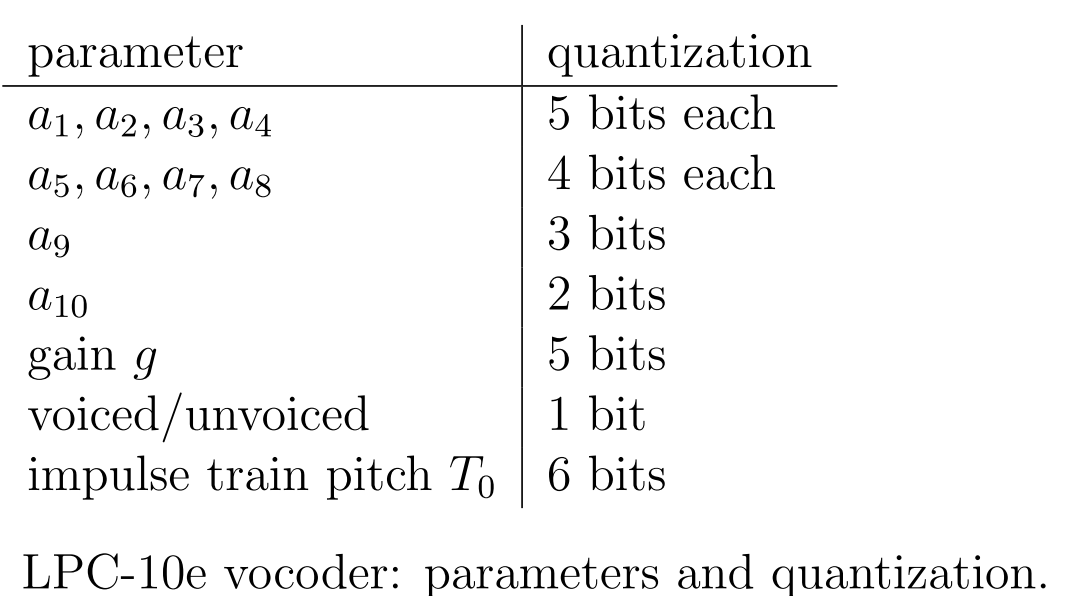
\includegraphics[width=\textwidth]{./images/lpc_10e}
\end{center}
\end{minipage}
Parameter $a_n$ müssen so gefunden werden, dass
\[ \hat{s}[n] = \sum_{k=1}^{P}a_ks_{in}[n-k] \]
möglichst nahe an $s_{in}[n]$ kommt. So ergibt sich:
\[ \textbf{R}_{ss} = \begin{bmatrix}
	\gamma_{ss}[0]	& \gamma_{ss}[1]	& \ldots	& \gamma_{ss}[P-1]\\
	\gamma_{ss}[1]	& \gamma_{ss}[0]	& \ldots	& \gamma_{ss}[P-2]\\
	\vdots			& \vdots			&			& \vdots\\
	\gamma_{ss}[P-1]& \gamma_{ss}[P-2]	& \ldots	& \gamma_{ss}[0]
\end{bmatrix}\]
\[ \textbf{r}_{ss} = \begin{bmatrix}
	\gamma_{ss}[1]\\
	\gamma_{ss}[2]\\
	\vdots\\
	\gamma_{ss}[P]
\end{bmatrix} \]
und
\[ \textbf{a} = \textbf{R}_{ss}^{-1}\textbf{r}_{ss} \]
Die Werte der Autokorrelation können angenähert werden durch
\[ \hat{\gamma}_{ss}[m] = \frac{1}{N-m} \sum_{n=1}^{N-m}s_{in}[n]s_{in}[n+m] \]
mit $N$ für die Anzahl Werte im Segment.\\
Der Fehler ist
\[ d[n] = s_{in}[n]-\hat{s}[n] \]
Die Verstärkung
\[ g=\sqrt{\frac{1}{N}\sum_{n=1}^{N}d^2[n]} \]
Durchschnittliche Amplituden Differenz Funktion (average magnitude difference
function):
\[ \bar{\gamma}_d[m]= \frac{1}{N-m} \sum_{n=1}^{N-m}\left|\frac{d[n]}{g} -
	\frac{d[n+m]}{g}\right| \] 
Wenn das minimum von $\bar{\gamma}_d[m]$ unter einen Schwellwert fällt, wird das
Segment als voice deklariert
\[ T_0 = \arg \min_{m\in[20,160]} \bar{\gamma}_d[m] \]

%===============================================================================
\section{LMS Algorithmus}
Passt seine Parameter stetig an.\\
Es wird der Eingangvektor und die Filterkoeffizienten benötigt
\[ \textbf{y}_n = \begin{bmatrix}y[n] \\ y[n-1] \\ \vdots \\ y[n-M]
	\end{bmatrix} \qquad \textbf{w} = \begin{bmatrix}
		w_0 \\ w_1 \\ \vdots \\ w_M	\end{bmatrix} \]
Der Ausgang wird berechnet mit
\[ \hat{s}[n] = \textbf{w}^T\textbf{y}_n \]
Der mittlere quadratische Fehler ist
\[ \varepsilon_{MSE}(\textbf{w}) = E \{ (\hat{s}[n]-s[n])^2 \} \]
Der Vektor \textbf{w} wird mit Nullen initialisiert und berechnet sich aus
\[ \textbf{w}^{(n+1)} = \textbf{w}^{(n)} + \underbrace{\mu\left( s[n] - 
	\left( \textbf{w}^{(n)}\right)^T\textbf{y}_n\right)\cdot\textbf{y}_n}_
	{=\textbf{w}_\Delta^{(n)}} \]
$\mu$ ist die Schrittweite und gibt an, wie oft der Algorithmus angepasst wird.
\begin{center}
	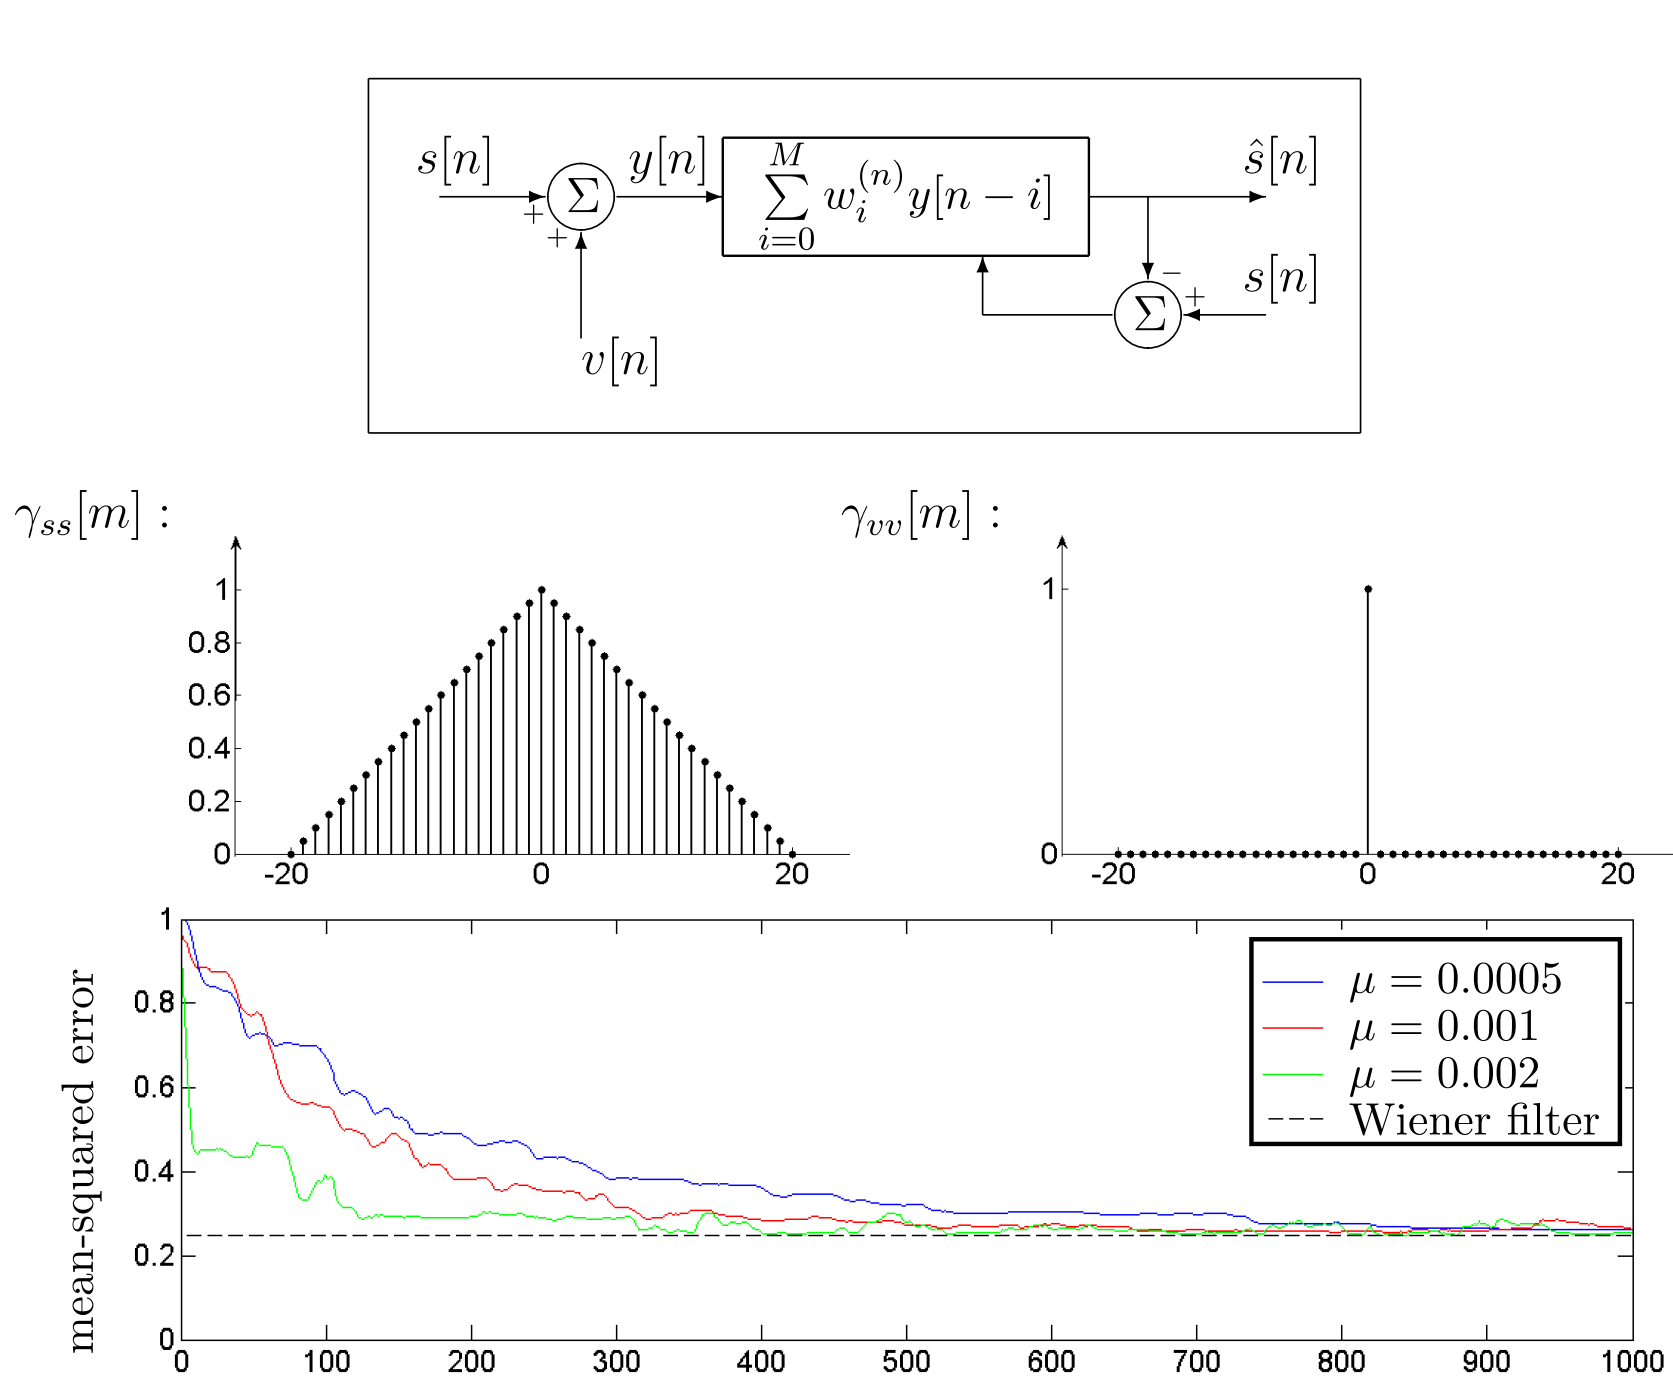
\includegraphics[scale=.7]{./images/lms_algorithm}
\end{center}